\section{1174069 - Fanny Shafira Damayanti}
\subsection{Teori}
\begin{enumerate}
	\item Jelaskan kenapa kata-kata harus di lakukan vektorisasi. Dilengkapi dengan ilustrasi atau gambar.
	\hfill\break
	Kata kata harus dilakukan vektorisasi dikarenakan atau bertujuan utk mengukur nilai kemunculan suatau kata yang serupa dari sebuah kalimat sehingga kata-kata tersebut dapat di prediksi kemunculanya. atau juga di buatnya vektorisasi data digunakan untuk memprediksi bobot dari suatu kata misalkan ayam dan kucing sama-sama hewan maka akan dibuat prediksi apakah kata tersebut akan muncul pada kalimat yang kira-kira memiliki bobot yang sama.
	\hfill\break
	\begin{figure}[H]
		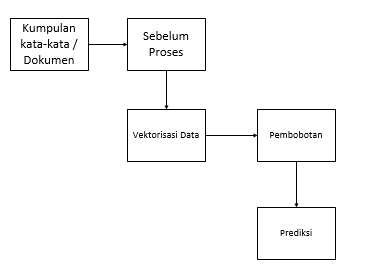
\includegraphics[width=4cm]{figures/1174069/5/1.png}
		\centering
		\caption{Teori 1}
	\end{figure}

	\item Jelaskan mengapa dimensi dari vektor dataset google bisa sampai 300. Dilengkapidengan ilustrasi atau gambar.
	\hfill\break
	Dimensi dataset dari google bisa mencapai 300 karena dimensi dari vektor tersebut digunakan untuk membandingkan bobot dari setiap kata, misalkan terdapat kata dog dan cat pada dataset google tersebut setiap kata tersebut di buat dimensi vektor 300 untuk kata dog dan 300 dimensi vektor juga untuk kata cat kemudian kata tersebt di bandingkan bobot kesamaan katanya maka akan muncul akurasi sekitar 70 persen kesamaan bobot dikarenakan kata dog dan cat sama sama di gunakan untuk hewan priharaan.
	\hfill\break
	\begin{figure}[H]
		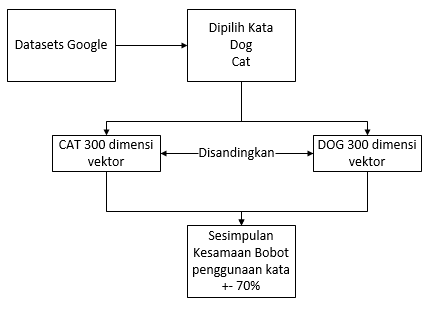
\includegraphics[width=4cm]{figures/1174069/5/2.png}
		\centering
		\caption{Teori 2}
	\end{figure}

	\item Jelaskan konsep vektorisasi untuk kata.dilengkapi dengan ilustrasi atau gambar.
	\hfill\break
	Vektorisasi untuk kata untuk mengetahui kata tengah dari suatau kalimat atau kata utama atau objek utama pada suatau kalimat contoh ( Jangan lupa subscribe channel saya ya sekian treimakasih ) kata tengah tersebut merupakan channel yang memiliki bobot sebagai kata tengah dari suatu kalimat atau bobot sebagai objek dari suatu kalimat. hal ini sangat berkaitan dengan dimensi vektor pada dataset google yang 300 tadi karena untuk mendapatkan nilai atau bobot dari kata tengah tersebut di dapatkan dari proses dimensiasi dari kata tersebut. 
	\hfill\break
	\begin{figure}[H]
		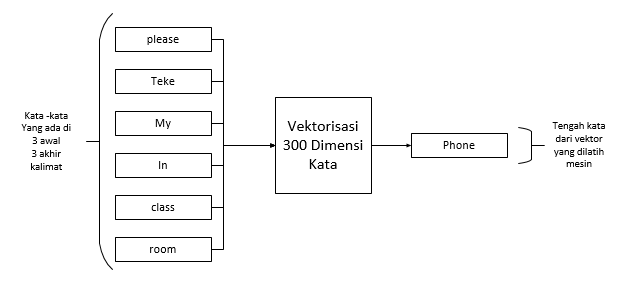
\includegraphics[width=4cm]{figures/1174069/5/3.png}
		\centering
		\caption{Teori 3}
	\end{figure}

	\item Jelaskan konsep vektorisasi untuk dokumen.dilengkapi dengan ilustrasi atau gambar.
	\hfill\break
	Vektorisasi untuk dokumen hampir sama seperti vektorisasi untuk kata hanya saja pemilihan kata utama atau kata tengah terdapat pada satu dokumen jadi mesin akan membuat dimensi vektor 300 untuk dokumen dan nanti kata tengahnya akan di sandingkan pada dokumen yany terdapat pada dokumen tersebut.
	\hfill\break
	\begin{figure}[H]
		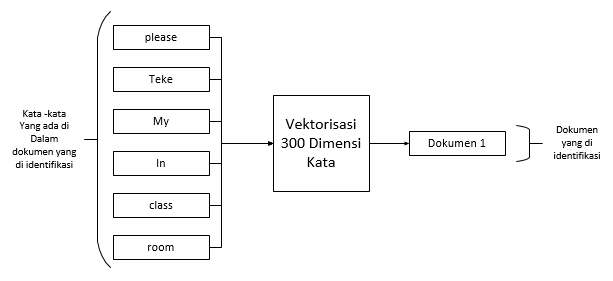
\includegraphics[width=4cm]{figures/1174069/5/4.png}
		\centering
		\caption{Teori 4}
	\end{figure}

	\item Jelaskan apa mean dan standar deviasi,dilengkapi dengan ilustrasi atau gambar.
	\hfill\break
	mean merupakan petunjuk terhadap kata-kata yang di olah jika kata kata itu akurasinya tinggi berarti kata tersebut sering muncul begitu juga sebaliknya, sedangkan setandar defiation merupakan standar untuk menimbang kesalahan. sehingga kesalahan tersebut di anggap wajar misarkan kita memperkirakan kedalaman dari dataset merupakan 2 atau 3 tapi pada kenyataanya merupakan 5 itu merupakan kesalahan tapi masih bisa dianggap wajar karna masih mendekati perkiraan awal.
	\hfill\break
	\begin{figure}[H]
		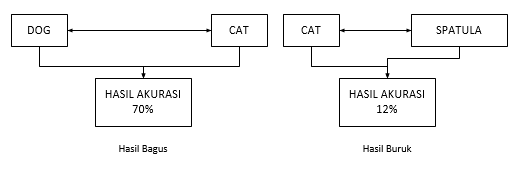
\includegraphics[width=4cm]{figures/1174069/5/5.png}
		\centering
		\caption{Teori 5}
	\end{figure}

	\item Jelaskan apa itu skip-gram,dilengkapi dengan ilustrasi atau gambar.
	\hfill\break
	Skip-Gram adalah kebalikan dari konsep vektorisasi untuk kata dimana kata tengah menjadi acuan terhadap kata kata pelengkap dalam suatu kalimat.
	\hfill\break
	\begin{figure}[H]
		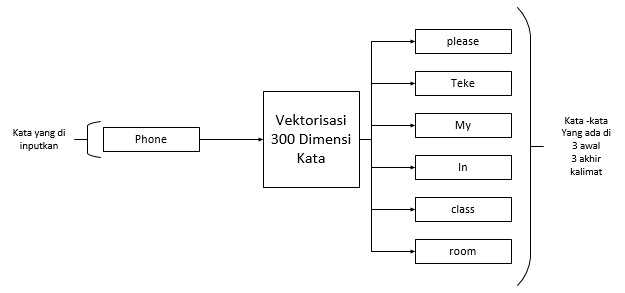
\includegraphics[width=4cm]{figures/1174069/5/6.png}
		\centering
		\caption{Teori 6}
	\end{figure}
\end{enumerate}
\subsection{Praktek}
\begin{enumerate}
	\item Cobalah dataset google, dan jelaskan vektor dari kata love, faith, fall, sick, clear,shine, bag, car, wash, motor, cycle dan cobalah untuk melakukan perbandingan similirati dari masing-masing kata tersebut.
	\begin{itemize}
		\item berikut merupakan code import gensim digunakan untuk membuat data model atau rangcangan data yang akan di buat. selanjutnya dibuat variabel gmodel yang berisi data vektor negativ. selanjutnya data tersebut di load agar data tersebut dapat di tampilkan dan di olah.
		\hfill\break
		\begin{figure}[H]
			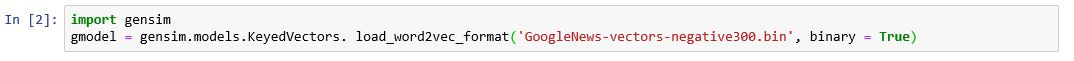
\includegraphics[width=4cm]{figures/1174069/5/7.jpg}
			\centering
			\caption{Praktek 1}
		\end{figure}
		\item berikut merupakan hasil lpengolahan kata love pada data google yang di load tadi. Sehingga memunculkan hasil vektor 300 dimensi untuk kata tersebut.
		\hfill\break
		\begin{figure}[H]
			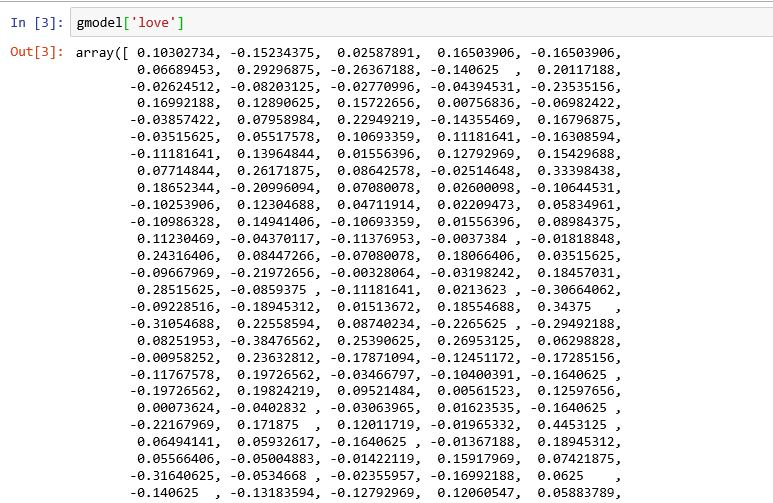
\includegraphics[width=4cm]{figures/1174069/5/8.jpg}
			\centering
			\caption{Praktek 1.1}
		\end{figure}
		\item berikut merupakan hasil lpengolahan kata faith pada data google yang di load. Sehingga memunculkan hasil vektor 300 dimensi untuk kata tersebut.
		\hfill\break
		\begin{figure}[H]
			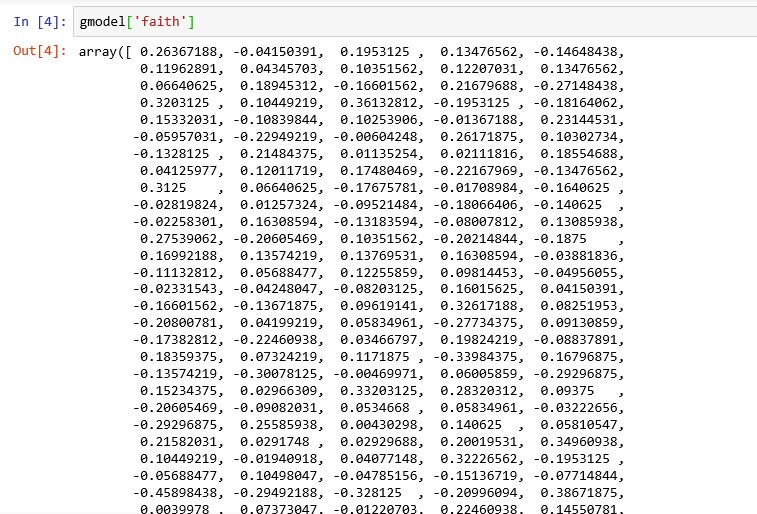
\includegraphics[width=4cm]{figures/1174069/5/9.jpg}
			\centering
			\caption{Praktek 1.2}
		\end{figure}
		\item berikut merupakan hasil lpengolahan kata fall pada data google yang di load. Sehingga memunculkan hasil vektor 300 dimensi untuk kata tersebut.
		\hfill\break
		\begin{figure}[H]
			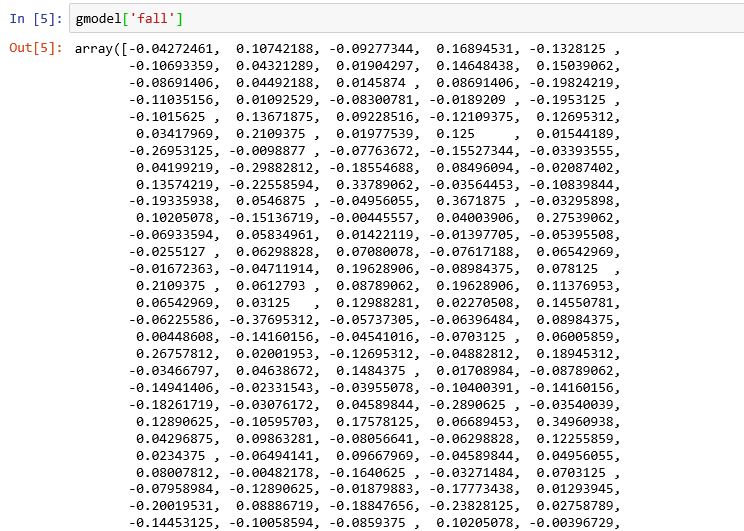
\includegraphics[width=4cm]{figures/1174069/5/10.jpg}
			\centering
			\caption{Praktek 1.3}
		\end{figure}
		\item berikut merupakan hasil lpengolahan kata sick pada data google yang di load. Sehingga memunculkan hasil vektor 300 dimensi untuk kata tersebut.
		\hfill\break
		\begin{figure}[H]
			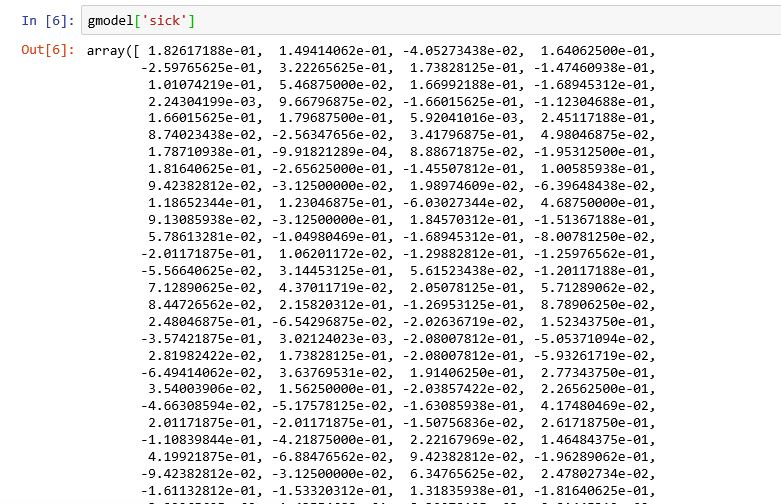
\includegraphics[width=4cm]{figures/1174069/5/11.jpg}
			\centering
			\caption{Praktek 1.4}
		\end{figure}
		\item berikut merupakan hasil lpengolahan kata clear pada data google yang di load. Sehingga memunculkan hasil vektor 300 dimensi untuk kata tersebut. 
		\hfill\break
		\begin{figure}[H]
			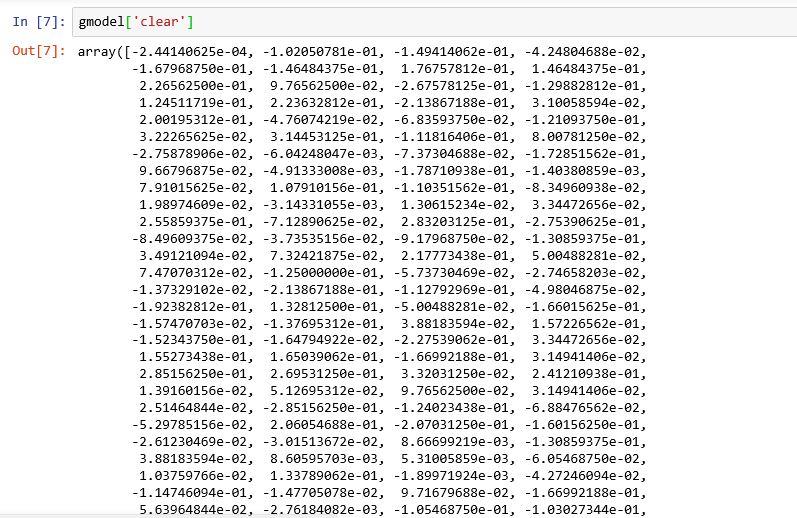
\includegraphics[width=4cm]{figures/1174069/5/12.jpg}
			\centering
			\caption{Praktek 1.5}
		\end{figure}
		\item berikut merupakan hasil lpengolahan kata shine pada data google yang di load. Sehingga memunculkan hasil vektor 300 dimensi untuk kata tersebut. 
		\hfill\break
		\begin{figure}[H]
			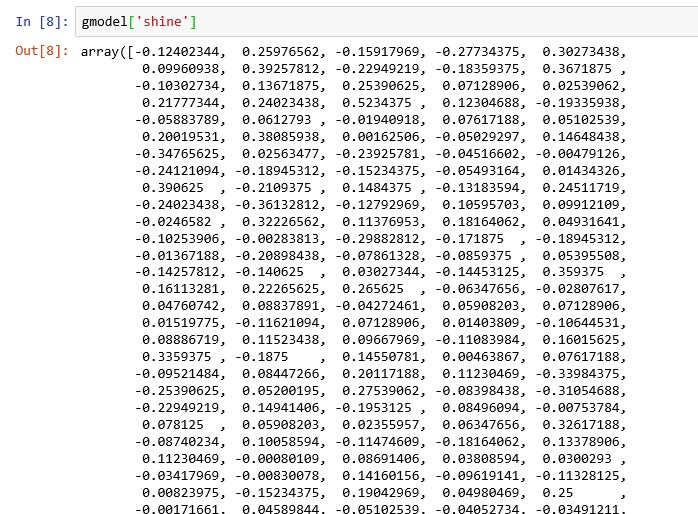
\includegraphics[width=4cm]{figures/1174069/5/13.jpg}
			\centering
			\caption{Praktek 1.6}
		\end{figure}
		\item berikut merupakan hasil lpengolahan kata bag pada data google yang di load. Sehingga memunculkan hasil vektor 300 dimensi untuk kata tersebut. 
		\hfill\break
		\begin{figure}[H]
			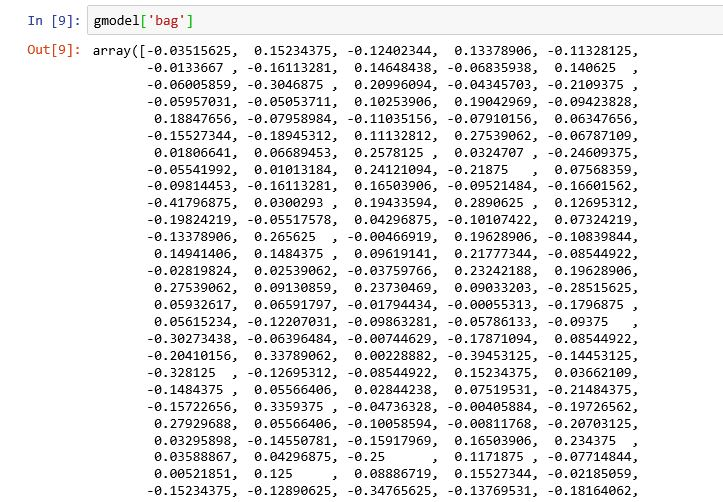
\includegraphics[width=4cm]{figures/1174069/5/14.jpg}
			\centering
			\caption{Praktek 1.7}
		\end{figure}
		\item berikut merupakan hasil lpengolahan kata car pada data google yang di load. Sehingga memunculkan hasil vektor 300 dimensi untuk kata tersebut. 
		\hfill\break
		\begin{figure}[H]
			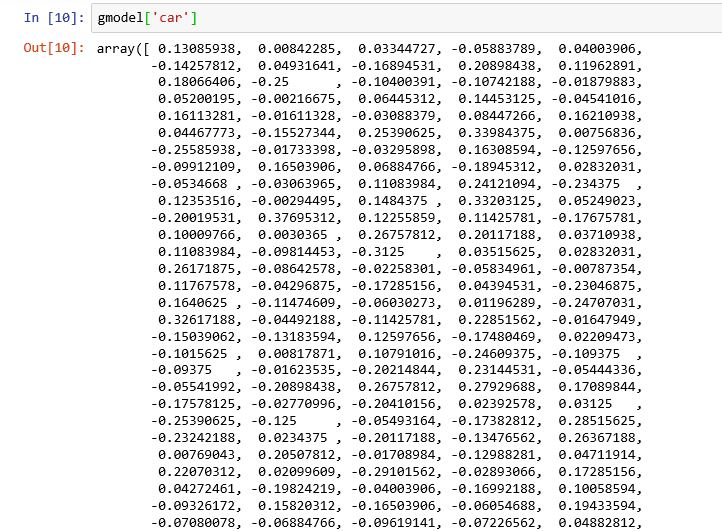
\includegraphics[width=4cm]{figures/1174069/5/15.jpg}
			\centering
			\caption{Praktek 1.8}
		\end{figure}
		\item berikut merupakan hasil lpengolahan kata wash pada data google yang di load. Sehingga memunculkan hasil vektor 300 dimensi untuk kata tersebut. 
		\hfill\break
		\begin{figure}[H]
			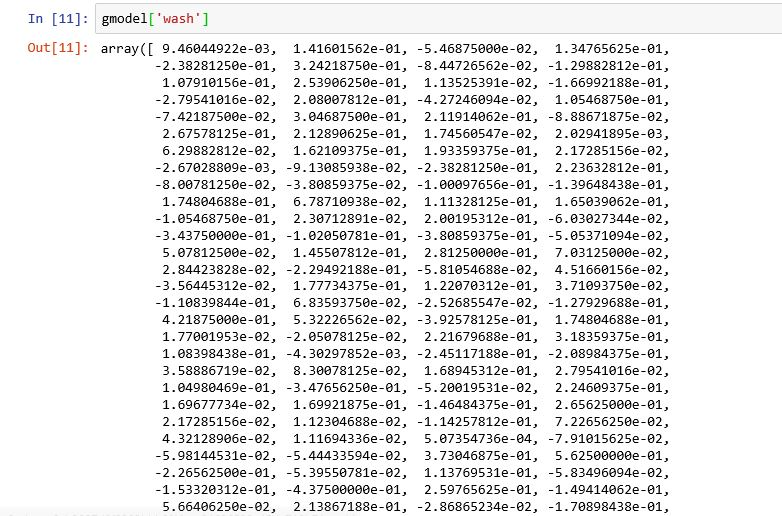
\includegraphics[width=4cm]{figures/1174069/5/16.jpg}
			\centering
			\caption{Praktek 1.9}
		\end{figure}
		\item berikut merupakan hasil lpengolahan kata motor pada data google yang di load. Sehingga memunculkan hasil vektor 300 dimensi untuk kata tersebut. 
		\hfill\break
		\begin{figure}[H]
			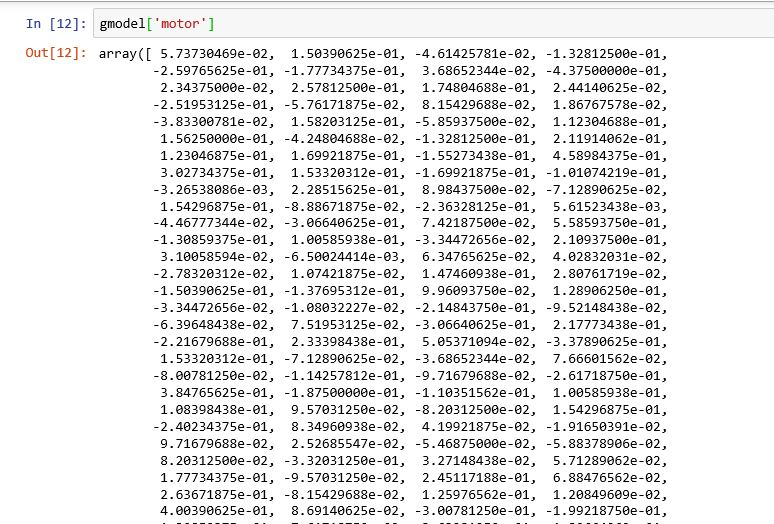
\includegraphics[width=4cm]{figures/1174069/5/17.jpg}
			\centering
			\caption{Praktek 1.10}
		\end{figure}
		\item berikut merupakan hasil lpengolahan kata cycle pada data google yang di load. Sehingga memunculkan hasil vektor 300 dimensi untuk kata tersebut. 
		\hfill\break
		\begin{figure}[H]
			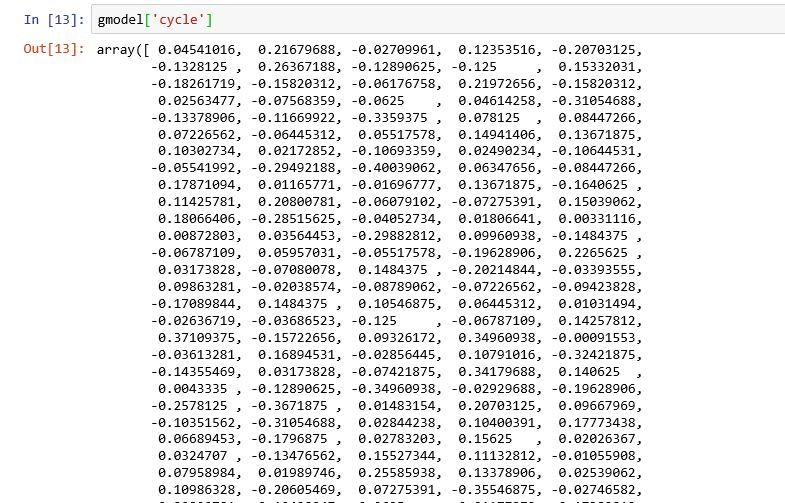
\includegraphics[width=4cm]{figures/1174069/5/18.jpg}
			\centering
			\caption{Praktek 1.11}
		\end{figure}
		\item berikut merupakan hasil dari similaritas kata kata yang di olah menjadi matrix tadi adapun persentase untuk perbandingan setiap katanya yaitu 9 persen untuk kata wash dan clear 7 persen untuk kata bag dan love 48 persen untuk kata motor dan car 12 persen untuk kata sick dan faith dan terakhir yaitu 6 persen untuk kata cycle dan shine.
		\hfill\break
		\begin{figure}[H]
			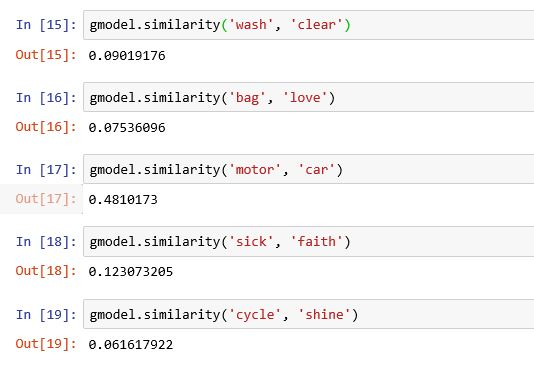
\includegraphics[width=4cm]{figures/1174069/5/19.jpg}
			\centering
			\caption{Praktek 1.12}
		\end{figure}
	\end{itemize}
	\item Jelaskan dengan kata dan ilustrasi fungsi dari extract words dan PermuteSentences
	\hfill\break
		\begin{figure}[H]
			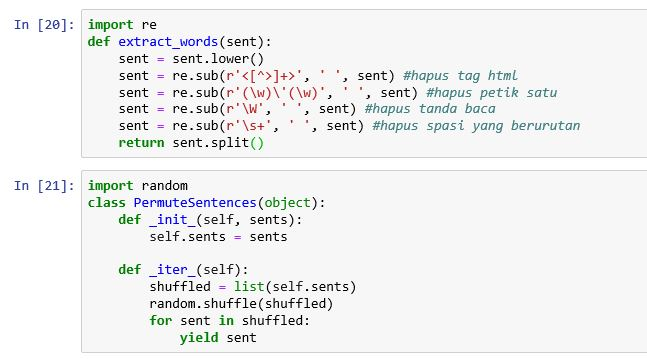
\includegraphics[width=4cm]{figures/1174069/5/20.jpg}
			\centering
			\caption{Praktek 2}
		\end{figure}
	\item Jelaskan fungsi dari librari gensim TaggedDocument dan Doc2Vec disertai praktek pemakaiannya.
	\hfill\break
		\begin{figure}[H]
			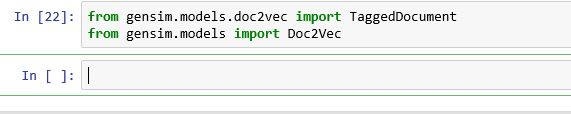
\includegraphics[width=4cm]{figures/1174069/5/21.jpg}
			\centering
			\caption{Praktek 3}
		\end{figure}
	\item Jelaskan dengan kata dan praktek cara menambahkan data training dari file yang dimasukkan kepada variabel dalam rangka melatih model doc2vac.
	\hfill\break
		\begin{figure}[H]
			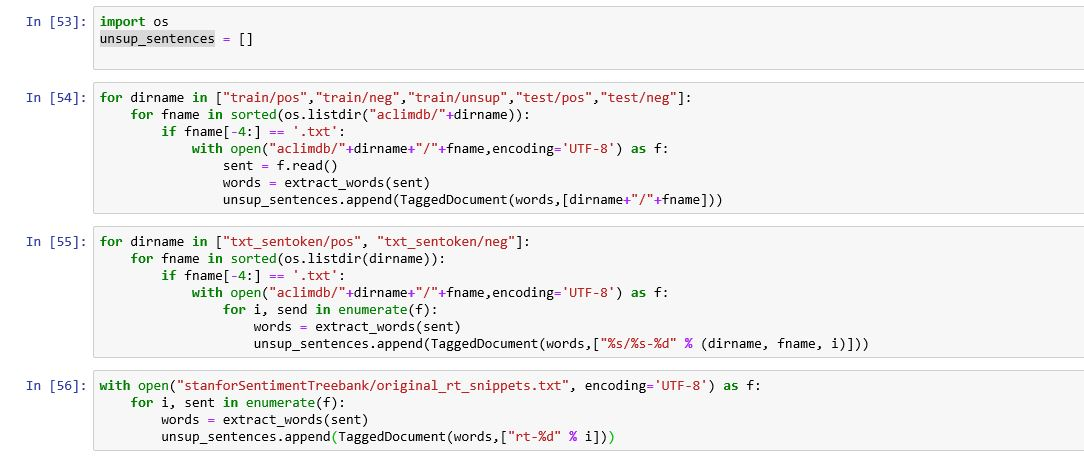
\includegraphics[width=4cm]{figures/1174069/5/22.jpg}
			\centering
			\caption{Praktek 4}
		\end{figure}
	\item Jelaskan dengan kata dan praktek kenapa harus dilakukan pengocokan dan pembersihan data.
	\hfill\break
		\begin{figure}[H]
			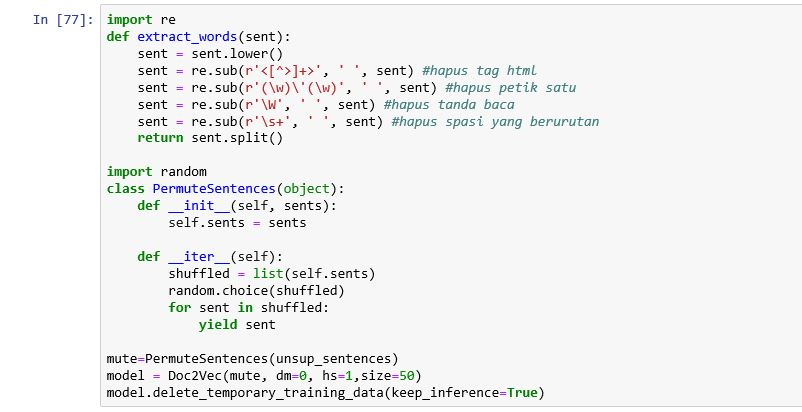
\includegraphics[width=4cm]{figures/1174069/5/23.jpg}
			\centering
			\caption{Praktek 5}
		\end{figure}
	\item Jelaskan dengan kata dan praktek kenapa model harus di save dan kenapa temporari training harus dihapus.
	\hfill\break
		\begin{figure}[H]
			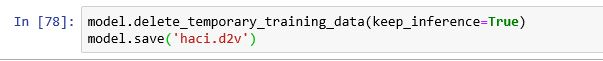
\includegraphics[width=4cm]{figures/1174069/5/24.jpg}
			\centering
			\caption{Praktek 6}
		\end{figure}
	\item Jalankan dengan kta dan praktek maksud dari infer code.
	\hfill\break
		\begin{figure}[H]
			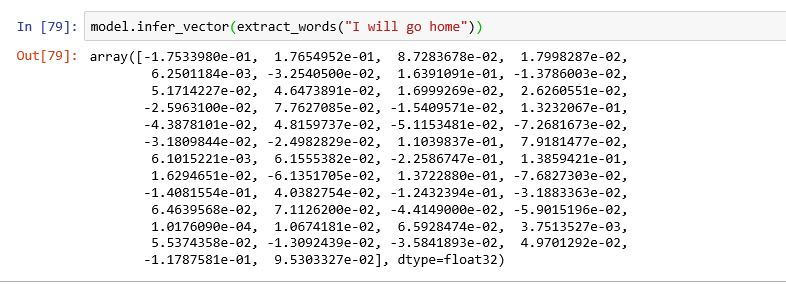
\includegraphics[width=4cm]{figures/1174069/5/26.jpg}
			\centering
			\caption{Praktek 7}
		\end{figure}
	\item Jelaskan dengan praktek dan kata maksud dari cosine similarity.
	\hfill\break
		\begin{figure}[H]
			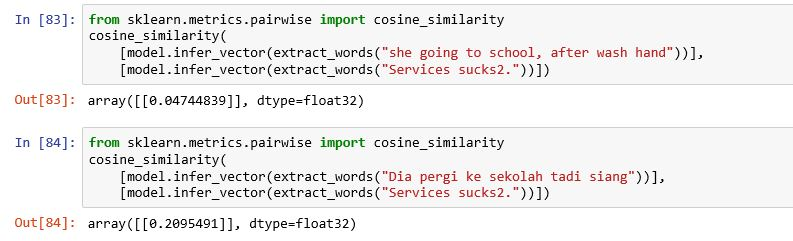
\includegraphics[width=4cm]{figures/1174069/5/27.jpg}
			\centering
			\caption{Praktek 8}
		\end{figure}
	\item Jelaskan dengan praktek score dari cross validation masing-masing metode.
	\lstinputlisting[firstline=8, lastline=27]{src/1174069/5/1174069.py}	
\end{enumerate}
\subsection{Penangan Error}
\begin{enumerate}
	\item SS Error
	\hfill\break
		\begin{figure}[H]
			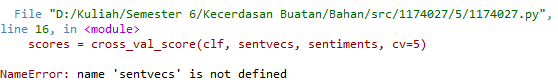
\includegraphics[width=4cm]{figures/1174069/5/error/5_name_error.png}
			\centering
			\caption{Name Error}
		\end{figure}
	\item Jenis error
	\begin{itemize}
		\item Name Error
	\end{itemize}
	\item Cara Penanganan
	\hfill\break
	Dengan Mengecek Kembali Baris Code Yang Dibuat
\end{enumerate}
\subsection{Bukti Tidak Melakukan Plagiat}
\hfill\break
\begin{figure}[H]
	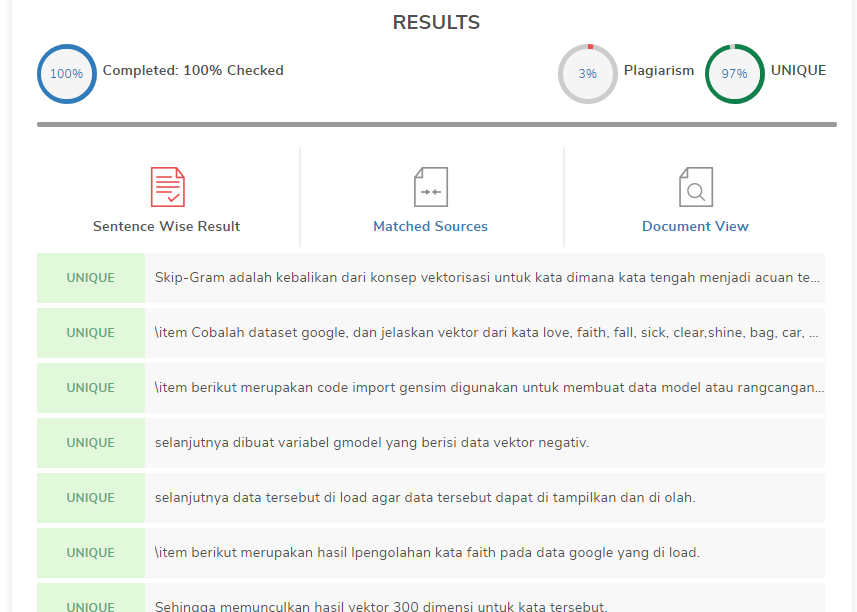
\includegraphics[width=4cm]{figures/1174069/5/bukti/bukti.PNG}
	\centering
	\caption{Bukti Tidak Melakukan Plagiat}
\end{figure}
\subsection{Link Youtube}
https://youtu.be/NKurTLe8MpI